\documentclass[11pt]{article}
\usepackage{amssymb}
\usepackage{amsthm}
\usepackage{enumitem}
\usepackage{amsmath}
\usepackage{bm}
\usepackage{adjustbox}
\usepackage{mathrsfs}
\usepackage{graphicx}
\usepackage{siunitx}

\title{\textbf{Solved selected problems of Classical Mechanics - Gregory}}
\author{Franco Zacco}
\date{}

\addtolength{\topmargin}{-3cm}
\addtolength{\textheight}{3cm}

\newcommand{\hatr}{\bm{\hat{r}}}
\newcommand{\hatth}{\bm{\hat{\theta}}}
\renewcommand*{\proofname}{Solution}

\begin{document}
\maketitle
\thispagestyle{empty}

\section*{Chapter 2 - Velocity, acceleration and scalar angular velocity}

	\begin{proof}{\textbf{2.3}} Given that acceleration is constant then the
        instant acceleration $a$ is equal to the average acceleration $a_{avg}$
        so assuming that we start from $t=0$ at $x=0$ and the final velocity
        is $v$ then we have that
        $$a = \frac{\Delta v}{\Delta t}$$
        $$a = \frac{v - u}{t - 0}$$
        $$at = v - u$$
        \begin{align}
            v = u + at
        \end{align}
        Now integrating both sides of the equation with respect to $t$:
        $$\int_0^t{vdt}=\int_0^t{udt}+\int_0^t{atdt}$$
        $$\int_{0}^t{dx}=\int_0^t{udt}+\int_0^t{atdt}$$
        $$x(t) - x(0) = ut + \frac{1}{2}at^2$$
        \begin{align}
            x = ut + \frac{1}{2}at^2
        \end{align}
        From (1) we get that $t = \frac{v-u}{a}$ and replacing in (2) we have
        $$x = u\frac{(v-u)}{a} + \frac{1}{2}a\frac{(v-u)^2}{a^2}$$
        $$ax = uv - u^2 + \frac{1}{2}(v^2 - uv + u^2)$$
        $$ax = \frac{v^2}{2} - \frac{u^2}{2}$$
        $$2ax = v^2 - u^2$$
        $$v^2 = u^2 + 2ax$$
        Finally if we replace $t=11.4~\si{s}$ and
        $v=116~\si{mph}=168.96\text{ ft/s}$ in (1) we get that
        $a = 14.82~\si{ ft/s^2}$ but then if we replace the same values in (2)
        assuming $x=0.25~\si{mi} =1320~\si{ft}$ we get that
        $a = 20.31~\si{ft/s^2}$ which means that the acceleration is not 
        constant because otherwise it must satisfy both equations.
    \end{proof}
    \begin{proof}{\textbf{2.6}}
        First we calculate the following
        \begin{equation*}
            \begin{split}
                r &= be^{\Omega t} \\
                \dot{r} &= b\Omega e^{\Omega t} \\
                \ddot{r} &= b\Omega^2 e^{\Omega t}
            \end{split}
            \quad\quad
            \begin{split}
                \theta &= \Omega t \\
                \dot{\theta} &= \Omega \\
                \ddot{\theta} &= 0 \\
            \end{split}
        \end{equation*}
        Now replacing in $\bm{v} = \dot{r}\hat{\bm{r}} +(r\dot{\theta})\hat{\bm{\theta}}$
        and in $\bm{a} = (\ddot{r} - r\dot{\theta}^2)\hat{\bm{r}} + (r\ddot{\theta} + 2\dot{r}\dot{\theta})\hat{\bm{\theta}}$
        we get that
        \begin{align*}
            \bm{v} = b\Omega e^{\Omega t}\hat{\bm{r}} +(be^{\Omega t}\Omega)\hat{\bm{\theta}}
        \end{align*}
        And
        \begin{align*}
            \bm{a} &= (b\Omega^2 e^{\Omega t} - b\Omega^2 e^{\Omega t})\hat{\bm{r}} + (be^{\Omega t}0 + 2b\Omega^2 e^{\Omega t})\hat{\bm{\theta}} \\
                   &= 2b\Omega^2 e^{\Omega t}\hat{\bm{\theta}}
        \end{align*}
        Then,
        \begin{align*}
            |v| &= \sqrt{2}b\Omega^2 e^{\Omega t} \\
            |a| &= 2b\Omega^2 e^{\Omega t}
        \end{align*}
        So by using the formula for the dot product we compute
        $cos(\alpha) = \frac{\bm{a} \cdot \bm{b}}{|a||b|}$ as
        \begin{align*}
            cos(\alpha) &= \frac{2b^2\Omega^3 e^{2\Omega t}}{(\sqrt{2}b\Omega^2 e^{\Omega t})(2b\Omega^2 e^{\Omega t})} \\
             &= \frac{1}{\sqrt{2}}
        \end{align*}
        Finally, this means that $\alpha = \pi / 4$.
    \end{proof}
\cleardoublepage
    \begin{proof}{\textbf{2.9}}
        From $\bm{v} = \dot{r}\hat{\bm{r}} +(r\dot{\theta})\hat{\bm{\theta}}$ we
        calculate the velocity vector where
        \begin{align*}
            \dot{r} &= \frac{2b}{\tau} - \frac{2b}{\tau^2}t \\
            \dot{\theta} &= \frac{1}{\tau}
        \end{align*}
        Then the velocity vector is
        \begin{align*}
            \bm{v} = \frac{2b}{\tau^2}(\tau - t)\hatr + \frac{bt}{\tau^3}(2\tau - t)\hatth
        \end{align*}
        Now let's compute $|\bm{v}|^2$
        \begin{align*}
            |\bm{v}|^2 &= \frac{4b^2}{\tau^4}\tau^2 - \frac{8b^2\tau}{\tau^4}t + \
                          \frac{4b^2}{\tau^4}t^2 + \frac{4b^2\tau^2}{\tau^6}t^2 - \
                          \frac{4b^2\tau}{\tau^6}t^3 + \frac{b^2}{\tau^6}t^4 \\
                       &= \frac{4b^2}{\tau^2} - \frac{8b^2}{\tau^3}t + \
                          \frac{8b^2}{\tau^4}t^2 - \frac{4b^2}{\tau^5}t^3 + \ 
                          \frac{b^2}{\tau^6}t^4 \\
                       &= \frac{b^2}{\tau^6}(t^4 - 4\tau t^3 + 8\tau^2 t^2 - \ 
                       8 \tau^3t + 4\tau^4)
        \end{align*}
        To find the maximum value of $|\bm{v}|$ let's consider the time
        derivative of $|\bm{v}|^2$
        \begin{align*}
            \frac{d|\bm{v}|^2}{dt} &= \frac{b^2}{\tau^6}(4t^3 - 12\tau t^2 + \ 
                                   16\tau^2 t - 8 \tau^3) \\
                                   &= \frac{4b^2}{\tau^6}(t^3 - 3\tau t^2 + \ 
                                   4\tau^2 t - 2\tau^3) \\
                                   &= \frac{4b^2}{\tau^6}(t^3 - \tau t^2 - \
                                   2\tau t^2 + 2\tau^2 t + 2\tau^2 t - 2\tau^3) \\
                                   &= \frac{4b^2}{\tau^6}(t(t^2 - 2\tau t + \ 
                                   2\tau^2)- \tau(t^2 - 2\tau t + 2\tau^2)) \\
                                   &= \frac{4b^2}{\tau^6}(t - \tau)(t^2 - \ 
                                   2\tau t + 2\tau^2)
        \end{align*}
        Since $t^2 - 2\tau t + 2\tau^2$ can be written as $\tau^2 + (t - \tau)^2$
        we see that this term no matter the value of $t$ is always positive so
        \begin{align*}
            \frac{d|\bm{v}|^2}{dt} = \begin{cases}
                <0 & \text{ if } t < \tau \\
                =0 & \text{ if } t = \tau \\
                >0 & \text{ if } t > \tau
            \end{cases}
        \end{align*}
        Hence $|\bm{v}|$ achives a minimum value when $t = \tau$ so
        $$|\bm{v}|^2 = \frac{b^2}{\tau^6}\tau^4$$
        $$|\bm{v}| = \frac{b}{\tau}$$
        Finally the acceleration is given by
        $$ \bm{a} = (-\frac{2b}{\tau^2} - \frac{2b}{\tau^3}t + \frac{b}{\tau^4}t^2) \hatr +\ 
        (\frac{4b}{\tau^2}(1 - \frac{t}{\tau}))\hatth$$
        and when $t = \tau$ we have that
        $$ \bm{a} = -\frac{3b}{\tau^2} \hatr$$
    \end{proof}
    \begin{proof}{\textbf{2.10}}
        The Lion's velocity can be calculated as
        $$\bm{v} = \dot{r}\hatr + r\dot{\theta}\hatth$$
        So calculating the speed of the Lion knowing that $\dot{\theta}$ is the
        angular velocity and can be written as $\dot{\theta} = \frac{u}{a}$
        where $u$ is the velocity of Daniel and $a$ is the radius then we get
        that
        \begin{align*}
            U^2 &= \dot{r}^2 + (r\dot{\theta})^2 \\
                &= \dot{r}^2 + (\frac{ru}{a})^2
        \end{align*}
        which can be re-written as
        \begin{align*}
            \dot{r}^2  &= U^2 - (\frac{ru}{a})^2 \\
                       &= \frac{u^2}{a^2}(\frac{U^2a^2}{u^2} - r^2)
        \end{align*}
        This ODE can be solved as follows
        $$\dot{r}  = \frac{u}{a}\sqrt{\frac{U^2a^2}{u^2} - r^2}$$
        $$\frac{dr}{dt} = \frac{u}{a}\sqrt{\frac{U^2a^2}{u^2} - r^2}$$
        $$\int{\frac{dr}{\sqrt{\frac{U^2a^2}{u^2}} - r^2}} = \int{\frac{u}{a}dt}$$
        $$\int{\frac{dr}{\sqrt{\frac{U^2a^2}{u^2}} - r^2}} = \frac{ut}{a}$$
        $$sin^{-1}(\frac{ur}{Ua}) + C = \frac{ut}{a}$$
        the constant of integration $C$ can be determined by knowing that $r=0$
        when $t=0$ then $C=0$ and therefore
        $$r = \frac{Ua}{u}sin(\frac{ut}{a})$$
        For $t = \pi a /2u$ we get that $r = Ua / u$ and if $U \geq u$ then
        $\frac{U}{u} \geq 1$ so $r = \frac{Ua}{u} \geq a$ which means that the
        Lion will caught Daniel in $t = \pi a /2u$ if $U \geq u$. \\
        In order to recognize the equation for $r$ as a circle we multiply both
        sides by $r$ so we get that 
        $$r^2 = \frac{Ua}{u}r\sin(\frac{ut}{a})$$
        now knowing that $r^2 = x^2 + y^2$ and that $r\sin(\frac{ut}{a}) = y$
        then
        $$x^2 + y^2 = \frac{Ua}{u}y$$
        $$y^2 - \frac{Ua}{u}y = -x^2$$
        $$y^2 - \frac{2Ua}{2u}y + (\frac{Ua}{2u})^2= -x^2 + (\frac{Ua}{2u})^2$$
        $$(y - \frac{Ua}{2u})^2 = -x^2 + (\frac{Ua}{2u})^2$$
        $$x^2 + (y - \frac{Ua}{2u})^2 = (\frac{Ua}{2u})^2$$
        which is an equation of a circle with center at $(0, \frac{Ua}{2u})$
        and radius $\frac{Ua}{2u}$.
        When $U = u$ we get that the Lion's path is described by
        $$x^2 + (y - \frac{a}{2})^2 = (\frac{a}{2})^2$$
        which is a circle with center at $(0, \frac{a}{2})$ and radius
        $\frac{a}{2}$.
    \end{proof}
    \begin{proof}{\textbf{2.11}}
        We know that the velocity in a general form can be written as
        $$\bm{v} = v \bm{t}$$
        where $\bm{t}$ is the unit tangential vector, and the acceleration can
        be written as
        $$\bm{a} = \frac{dv}{dt}\bm{t} + \frac{v^2}{\rho}\bm{n}$$
        where $\bm{n}$ is the unit normal vector, since $v$ is constant
        then $\frac{dv}{dt}=0$ so the acceleration can be written as
        $$\bm{a} = \frac{v^2}{\rho}\bm{n}$$
        which only has the normal component, therefore the acceleration is
        perpendicular to the velocity.
    \end{proof}
    \begin{proof}{\textbf{2.14}}
        Knowing that
        $$r = b \cosh(\Omega t)$$
        then
        $$\dot{r} = b \Omega\sinh(\Omega t)$$
        $$\ddot{r} = b \Omega^2\cosh(\Omega t)$$
        so from the polar velocity equation we have that
        \begin{align*}
            \bm{v} &= \dot{r}\hatr + r\dot{\theta}\hatth \\
                   &= b \Omega\sinh(\Omega t) \hatr + b \Omega\cosh(\Omega t) \hatth \\
                   &= b \Omega(\sinh(\Omega t) \hatr + \cosh(\Omega t) \hatth) 
        \end{align*}
        and the speed of the particle is then
        \begin{align*}
            |v|^2 &= b^2\Omega^2\sinh^2(\Omega t) + b^2 \Omega^2\cosh^2(\Omega t) \\
                  &= b^2\Omega^2 \cosh(2 \Omega t)
        \end{align*}
        Finally, the acceleration is derived as follows
        \begin{align*}
            \bm{a} &= (\ddot{r} - r\dot{\theta}^2) \hatr + (r\ddot{\theta} + \ 
                    2\dot{r}\dot{\theta}) \hatth \\
                   &= [b \Omega^2\cosh(\Omega t) - b \Omega^2\cosh(\Omega t)] \hatr + \
                    [0 + 2 b \Omega^2\sinh(\Omega t)] \hatth \\
                   &= 2 b \Omega^2\sinh(\Omega t) \hatth
        \end{align*}
        Therefore the acceleration direction is circunferential and is
            given by $\hatth$.
    \end{proof}
    \begin{proof}{\textbf{2.18}}
        As the graph shows P is at $(b \sin(\Omega t), 0)$ from there and by
        using Pythagoras theorem we can derive that Q is at
        $(0, \sqrt{a^2 - b^2 \sin^2(\Omega t)})$ then C, the center
        of the link, has coordinates given 
        $(\frac{b}{2}\sin(\Omega t), \frac{\sqrt{a^2 - b^2 \sin^2(\Omega t)}}{2})$.
        If we now move the origin $(0, 0)$ to C then the coordinates of P are
        given by $(\frac{b}{2}\sin(\Omega t), -\frac{\sqrt{a^2 - b^2 \sin^2(\Omega t)}}{2})$
        so we have that the sine of the angle between the link and the negative
        Y-axis is given by  
        $$\sin(\theta) = \frac{\frac{b}{2}\sin(\Omega t)}{\frac{a}{2}} \quad\text{ so }\quad
        \theta = \sin^{-1}\left(\frac{b \sin{\Omega t}}{a}\right)$$
        now derivating this expression with respect to $t$ we get the Angular 
        velocity as
        $$\dot{\theta} = \omega = \frac{b\Omega\cos(\Omega t)}{\sqrt{a^2 - b^2\sin^2(\Omega t)}}$$
        Finally, since we know the coordinates for C we can calculate the
        velocity as
        \begin{align*}
            \bm{v} = \frac{\Omega b}{2}\cos(\Omega t) \bm{i} - \ 
            \frac{\Omega b^2 \sin(\Omega t) \cos(\Omega t)}{2\sqrt{a^2 - b^2 sin^2(\Omega t)}} \bm{j} 
        \end{align*}        
        so now we can calculate the speed for the link center by  
        \begin{align*}
            |v|^2 &= \frac{\Omega^2b^2}{4}\cos^2(\Omega t) + \
            \frac{\Omega^2 b^4 \sin^2(\Omega t) \cos^2(\Omega t)}{4(a^2 - b^2 sin^2(\Omega t))} \\
                  &= \frac{\Omega^2b^2}{4}\cos^2(\Omega t) \left(1 + \ 
                  \frac{b^2 \sin^2(\Omega t)}{a^2 - b^2 sin^2(\Omega t)}\right) \\
                  &= \frac{\Omega^2b^2}{4}\cos^2(\Omega t) \left( \ 
                  \frac{a^2}{a^2 - b^2 sin^2(\Omega t)}\right) \\
                  &= \frac{\Omega^2b^2a^2 \cos^2(\Omega t)}{4(a^2 - b^2 sin^2(\Omega t))}
        \end{align*}
        Finally
        $$|v| = \frac{\Omega ba\cos(\Omega t)}{2\sqrt{a^2 - b^2 sin^2(\Omega t)}}$$
    \end{proof}
    \begin{proof}{\textbf{2.22}}
        \item[(i)]
        Solving the equations given by computational means (Runge-kutta method)
        $$\dot{X} = -\frac{v^D X}{\sqrt{X^2 + Y^2}} - v^H_x \quad \quad \ 
          \dot{Y} = -\frac{v^D Y}{\sqrt{X^2 + Y^2}} - v^H_y$$
        when $v^D = v^H$ we get the following plot\\
        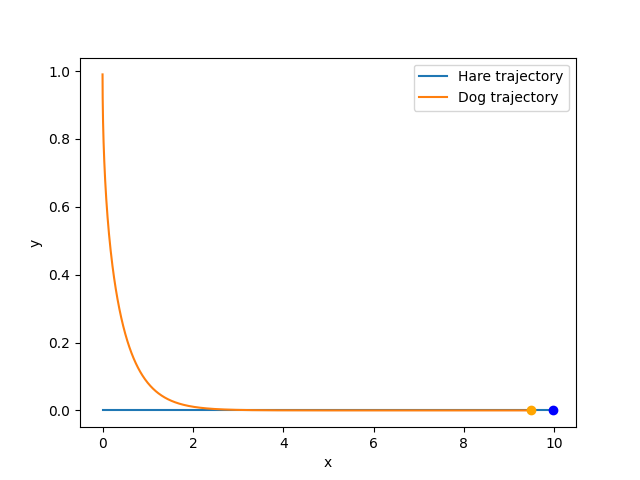
\includegraphics{gregory-2.22-1_vd=vh.png}
\cleardoublepage
        but if $v^D > v^H$\\
        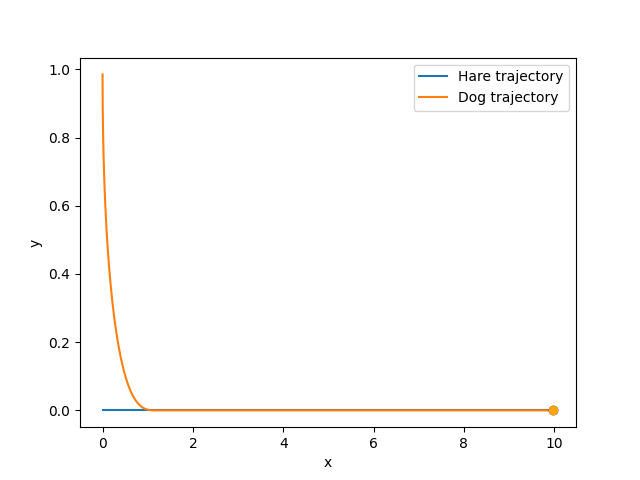
\includegraphics{gregory-2.22-1_vd>vh.png}
\cleardoublepage        
        \item[(ii)]
        Now we solve the equations for the case where the Hare has a circular
        trajectory
        when $v^D = v^H$ we get the following plot\\
        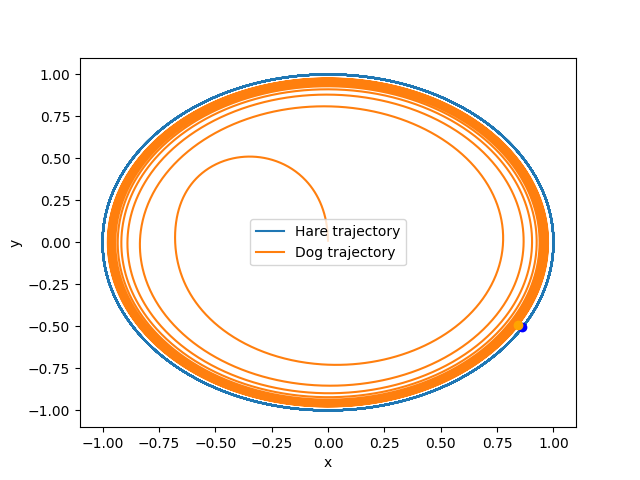
\includegraphics{gregory-2.22-2_vd=vh.png}
\cleardoublepage
        but if $v^D > v^H$\\
        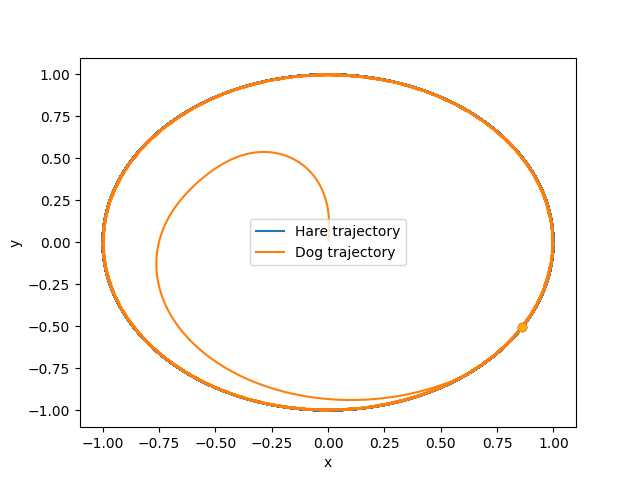
\includegraphics{gregory-2.22-2_vd>vh.png}
          
    \end{proof}

\end{document}























